\documentclass{llncs}
%
\usepackage[UTF8]{ctex}
\usepackage{amsfonts}
\usepackage{amstext}
\usepackage{amsmath}
\usepackage{enumitem}
\usepackage{multirow}
\usepackage{graphicx}
\usepackage[center]{subfigure}
\usepackage{amssymb}
\usepackage{graphicx,amsmath} % Add all your packages here
\usepackage{subfigure}
\usepackage{algorithm}
\usepackage{algorithmic}
\renewcommand{\algorithmicrequire}{ \textbf{Input:}}
\renewcommand{\algorithmicensure}{ \textbf{Output:}}
\usepackage{url}
\usepackage{cite}
\usepackage{color}
%
\begin{document}
	
\title{现实的未来: 基于人工智能的混合现实}
\author{Anynimous}
\institute{School of Computer Science and Engineering, Beihang University, Beijing, China\\
%	\email{\{moyuanhuang, w.rong, jiangnan, xiongz\}@buaa.edu.cn}\\
%	\and Department of Computer Science, University of Victoria, Victoria, Canada\\
%	\email{tom.arjannikov@gmail.com}
}
\maketitle

\begin{abstract}
将虚拟现实(VR)和增强现实(AR)带入现实世界当中已不再是新鲜的研究题目。 虚拟现实与增强现实均可在大多数现代技术相关设施中找到,例如医院中的医疗设备,电影制作中人与3D模型的合体,热门游戏(如安卓系统中的Pokemon GO游戏--使用了增强现实(AR)技术),日常工具等。然而,当前的虚拟现实和增强现实技术只是简单的技术,仅为我们的日常工作与生活带来更多便利, 这意味着它们只是一些与PC没有本质区别的工具。 为了让虚拟现实以及增强现实可以在现实世界中有更大的意义与发展,人们也已经开始将人工智能和虚拟世界融合在一起。在本论文当中我们将探讨基于人工智能的人造现实,创造一个真正的混合现实世界,并将人们能真正地与这些虚拟世界里的物体有着实际的互动。

\keywords{混合现实,扩展现实,人工智能,虚拟现实,增强现实}
\end{abstract}

\section{绪论}

\begin{figure}[h!]
	\centering
	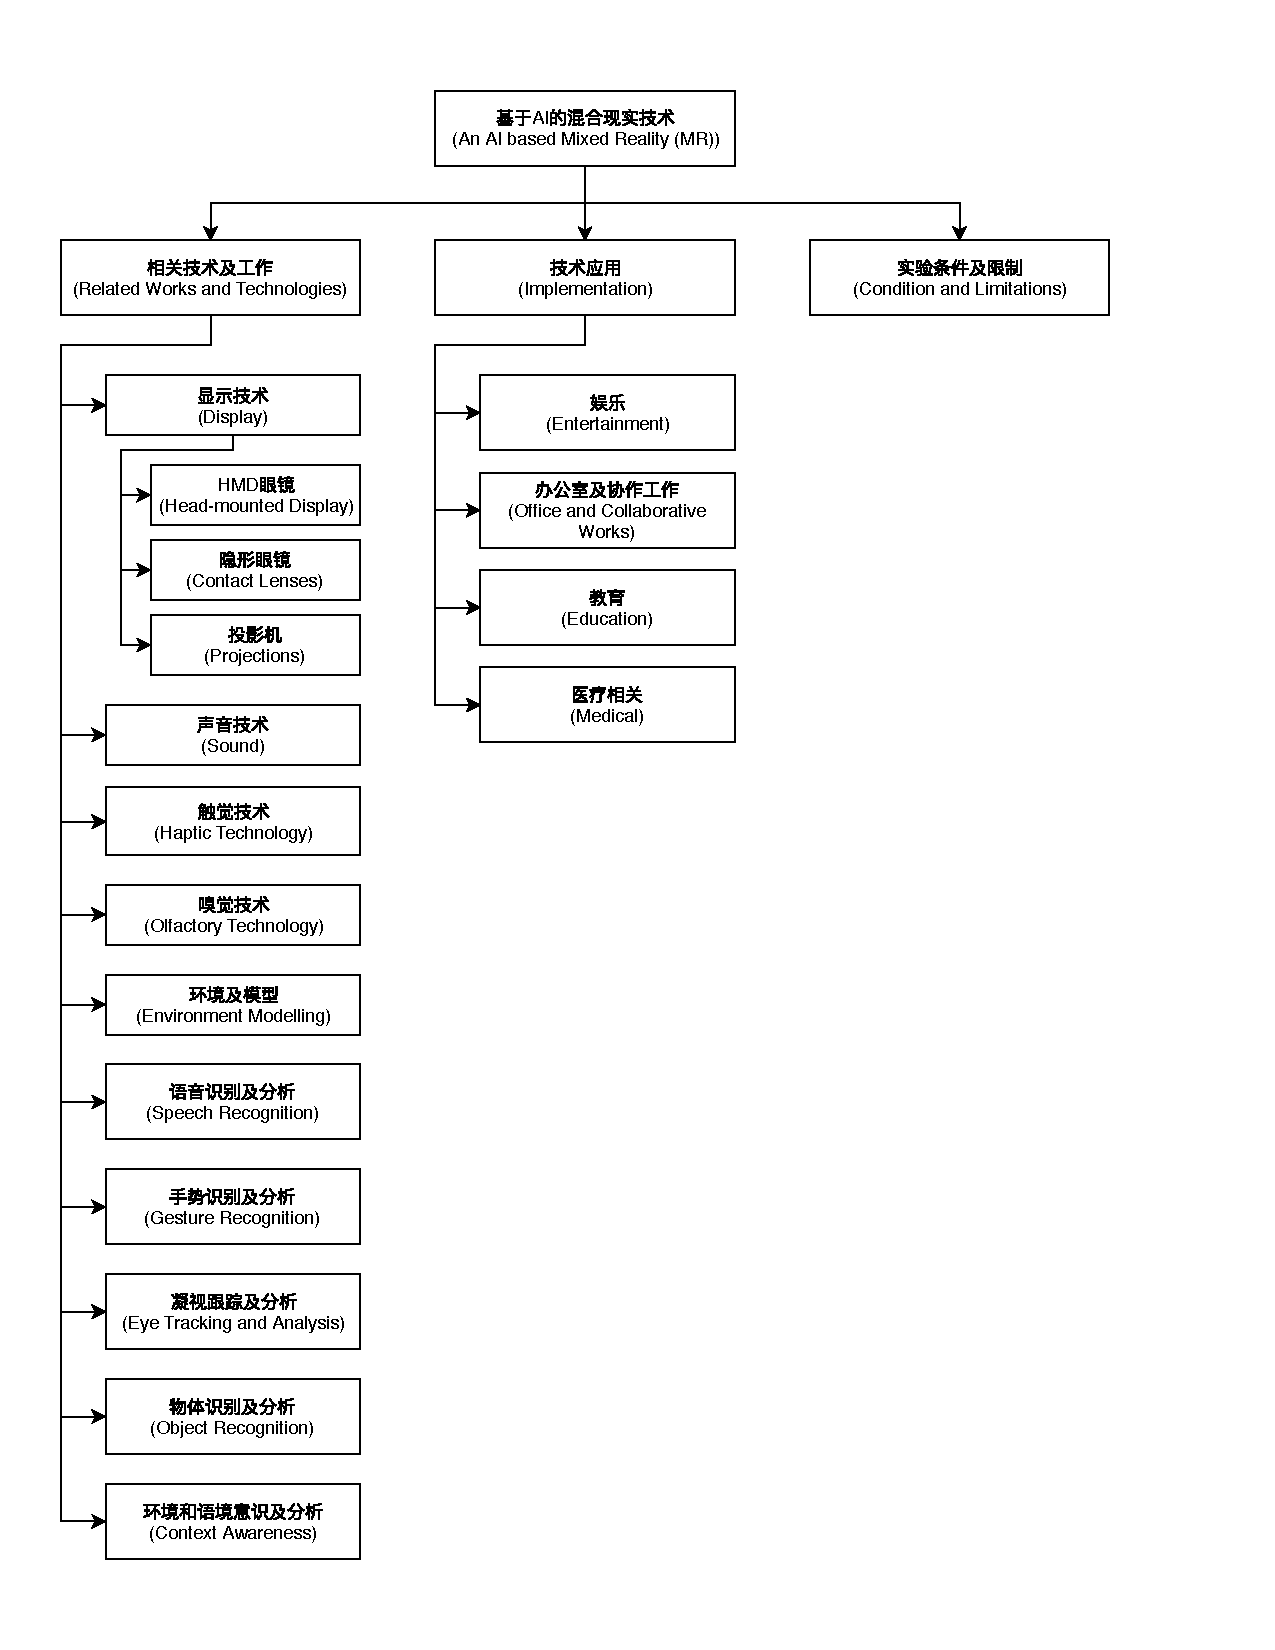
\includegraphics[width=1\linewidth]{figures/summary}
	\caption{综述模型图}
	\label{fig:summary}
\end{figure}

在当今世界当中--也可能在未来的几十年--我们的现实世界将成为我们称之为扩展现实(XR)的世界。 扩展现实本身的含义是一种新型的混合现实,它将虚拟现实(VR),增强现实(AR)以及混合现实(MR)融合在一起,制造一个链接虚拟和现实世界的一条“线”\cite{mann2018all}。 我们不得不承认,我们所谓的现实世界已不像之前一般“纯洁”,其中多多少少存在着虚拟物体的分子,因为我们的世界不断与虚拟现实,增强现实等人造现实的存在相结合,制造一个混合现实。 在这些多种类型的现实中,VR和AR扮演着主要角色。他们是多种现实中带头的两大虚拟世界技术,涵盖了我们当前的大部分技术,无论是电影制作,游戏开发,医疗设施等。

有了虚拟现实与增强现实的技术其实将虚拟世界与现实世界融合在一起是指日可待。不过目前的技术还有许多不便,不仅如此,虚拟现实技术并非所有人都花得起的,因为它的必需品便是虚拟现实眼睛(如Oculus Rift等设备)而正是此设备的价格相对比较高。好在增强现实正好与虚拟现实相反,有着一个手机,下载软件便可享受增强现实的技术。不过这两个不足以把虚拟世界与现实世界融合在一起,因为不论哪一个都有自己的不足。

除此之外,一个没有智能的虚拟世界全然与硬编码系统电脑并没有多大区别,它只能成为人们用的一个工具而不能真正与人们交流及互动。最好的例子便是游戏中的角色,一般的游戏并没有人工智能(AI)技术在其中,所有的交流,人物角色说的话,用户能说的话都是固定的,他们并不会识别出这些固定定义之外的事情,如用户的感情等信息。本论文的目的是讨论如何将一个有智能的虚拟物体(如人物)带到显示世界当中与人们交流。

\subsection{VR,AR,MR的定义}
相信VR(虚拟现实)和AR(增强现实)在人们的耳朵里已经不是陌生的俗语了。如今许多游戏都使用VR技术,就连看电影也可以使用VR的设备(如Oculus Rift等设备)。Oculus Rift是在2014年3月被Facebook收购了\cite{hoffman2014feasibility}。

当然,AR技术在人们生活中混的也不错。不仅有AR游戏,AR还存在别的方面。AR技术最初的模样就是Virtual Fixture。它是在1992年由Louis Rosenberg在USAF Armstrong Labs开发的\cite{DBLP:conf/vr/Rosenberg93a}。

由于定义上的相似性,许多人无法分辨出在虚拟现实和增强现实之间存在差异。 然而,它们在行动中确实有着巨大的差异。虚拟现实的含义是将我们的“现实世界”(用户的视觉知觉等)带入虚拟世界,而增强现实的工作原理完全与虚拟现实相反,它是将虚拟世界带到人们所谓的现实世界\cite{feiner1993knowledge}。

对于一般的虚拟现实技术来说有以下几个特点:
\begin{enumerate}
	\item 技术本身只会对你的视觉,听觉产生影响,并不包括嗅觉与触觉这两个知觉
	\item 能将用户带到一个完整的世界,完整的场景与画面
	\item 一旦带上VR眼镜,用户基本与现实世界“断了链接”,对现实世界没有意识
	\item 单反是两个人带着VR眼镜进入同一个世界里,他们两个将看到的东西是一致的
\end{enumerate}

而对于增强现实技术来说有以下几个特点:
\begin{enumerate}
	\item 画面完全只会在设备中显示,对人的知觉并没有任何影响
	\item 显示出的虚拟世界分子只是一小部分,并不会带来巨大或者多数的虚拟物体
	\item 使用的过程当中,用户仍然会对虚拟世界以及现实世界两个世界有意识
	\item 虚拟世界与现实世界可以说是完全隔开的,用户只能在设备中(手机)看到虚拟世界的内容,比如把手机摄像头向着某个食物会使手机中出现该食物的相关信息。除非别人也看着你的手机,或者用着自己的手机也同样向着那食物,用户与其他人所看到的画面并不一致
\end{enumerate}

\begin{table}
	\centering
	\caption{虚拟现实与增强现实的对比}
	\label{tb:vr-ar-difference}
	\begin{tabular}{|c|c|c|}
		\hline
		\textbf{特点}               &
		\textbf{VR}               & 
		\textbf{AR}         \\ \hline
		对知觉的影响 & 视觉,听觉,手势
		& 视觉,听觉          \\ \hline
		工作原理 & 用户进入完整的虚拟世界               & 虚拟物体进入现实世界                               \\ \hline
		对现实的意识 & 隔开               & 融合                 \\ \hline
	\end{tabular}
\end{table}

\begin{figure}
	\centering
	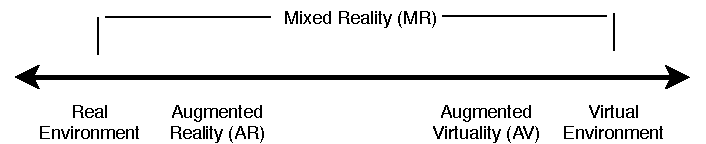
\includegraphics[width=0.7\linewidth]{figures/virtual_continuum}
	\caption{现实-虚拟连续体}
	\label{fig:virtualcontinuum}
\end{figure}

由图\ref{fig:virtualcontinuum}可看到AR,VR,MR的大概的区别。混合现实(MR)的含义是结合虚拟现实与增强现实的技术,把现实世界与虚拟世界结合在一起\cite{milgram1994taxonomy},使人造现实可以更完整,因为由表\ref{tb:vr-ar-difference}已经可以看到VR和AR虽然均会对人们的视觉与听觉产生影响但是VR对人的影响是完全环绕的,换句话说是可以让用户觉得自己就在那个虚拟世界里,而AR虽然也会有显示和声音但那只不过是手机上普通显示与声音。MR的意义是将AR的技术带进VR眼睛里,使虚拟和现实世界相结合但有着VR技术所有的环绕显示与声音。

\subsection{AI与人造现实}
首先,在现代的生活当中已经越来越常见了。不论是娱乐,机器人,手机或电脑助手等等都有着一些简单的人工智能。虽如此,人工智能对大多人们的生活还未有大的影响,就算有人工智能技术的设备也都只是一些简单的人工智能,比如推荐系统,聊天软件,情感分析等。

未来在虚拟世界与现实世界的结合中难免也会把人工智能插进去。在目前混合世界的发展还未成熟时,我们在此人造技术中常见的就是一些简单的工具,把电脑和手机上的工具带入两个世界结合的边界中,故此并没有人工智能技术在其中。

那该如何将AI与人造显示积极地结合在一起呢?最简单的例子可以从游戏系统看到,因为游戏本身是尽量模拟现实世界的一切。比如制造一个有着智能的虚拟人物,这个虚拟人物可以在人的生活当中扮演多种角色如助理,朋友,老师,等。总的来说是完全制造一个完整的虚拟世界然后再将那虚拟世界与现实世界结合,而不仅仅简单地把虚拟工具带到现实当中。

\

\section{相关工作}

想要将虚拟世界和现实世界结合成为混合现实原本已经不是一个简单的任务,我们需要考虑的很全面。因为想要让人们觉得以及“相信”那些虚拟世界首次需要让人的眼睛与耳朵相信,于是需要一个环绕的显示与声音技术。其次还可以加上人们的嗅觉和触觉。而在AI方面,“智能”是包括对某物体周围的环境,东西,情况都有着意识并能分析当时所“看到”的一切。

\subsection{显示}

混合现实的显示技术是可以通过很多设备实现的。我们知道VR使用的是Head-mounted Display (HMD)\cite{hoellwarth2015head},是一个头戴式的大眼镜,此VR眼镜不仅包括显示技术也包括声音技术,实现一个环绕的环境。一旦用户带上VR眼镜,他们将会被带进虚拟世界里,此时对现实世界并没有任何意识。自然有自己的危险,因为这样用户没法知道自己走到哪儿了,前面是否有障碍或者危险。

与VR相反的AR只是用手机这种设备显示虚拟世界的内容。他不会成为人们与现实世界的障碍但也不能让人们“相信”那些虚拟世界里的内容,因为用户智能在手机屏幕看到虚拟世界,也只能从手机或耳机听到虚拟世界里的声音,这跟看电影玩游戏并没有任何区别。他唯一与现实世界的关联就是在手机屏幕上产生的虚拟物体是与现实世界中被摄像头拍到的东西有关,只是结合结果智能在手机里出现\cite{cohen2009interactivity}。

\subsubsection{眼镜}
混合现实既然是把VR和AR结合在一起,在视觉方面自然是要让用户可以看到全面的画面(VR技术)但是同时也仍然可以看到现实世界中的环境(AR技术)。故此,微软已经有一个叫做Windows Mixed Reality的产品。还有另一种解决方案就是让MR HMD眼镜可以透视\cite{DBLP:conf/ismar/ZhouDB08}。这些设备使用的方式是类似于VR头戴式眼镜\cite{kress2019mixed}。带上之后自然有着环绕的环境,只是缺点就是这种眼镜不仅重而且也不方便。要是想要真正把虚拟世界带到人们的生活当中,若需要每个人天天都带着那么大的眼镜会妨碍很多事\cite{olshannikova2015visualizing}。

\subsubsection{隐形眼镜}
与眼镜相似的设备就是隐形眼镜。它们两个的区别就如同普通的眼镜与隐形眼镜,带上去之后隐形眼睛可以让戴上它的人不觉得有任何障碍,在外面的人眼里也不会看到任何异处。目前这种可以显示虚拟世界的隐形眼镜还在开发中,完全还未成熟,也并没有很多人知道这个技术。隐形眼镜的缺点就在于声音不能放在同一个设备里,必须带上耳机才能听到声音。

\subsubsection{投影}
显示虚拟物体的另一种方式就是通过投影机。如果你们看过Jurassic Park电影,里面的一个恐龙博物馆使用投影机将恐龙的模型投影出,就如同那个恐龙就站在人们中间。使用投影机的优点就是每个人都可以看到虚拟物体,不需要通过任何设备,可以直接看到。缺点就在于,如果要做一个比较大的虚拟环境以及多数虚拟物体,开销自然会很大,安装也比较麻烦。只不过,这种投影机就算不能完全替代MR眼镜,却可以兼用。

\subsection{声音}
声音方面就简单多了,因为我们现在的耳机甚至已经可以完全让用户无法听到外面的声音,更别说环绕声音。可以提高的方面就是让耳机带上去可以更方便,尤其要跟MR眼镜兼用。第一种方式就是与大的MR眼镜放在一块儿,这与当前的VR眼镜以及MR眼镜一样。另一种方式就是使用普通的耳机。这种方式适合MR隐形眼镜。

\subsection{触觉}
触摸包括两大部分:人的触觉以及触摸对虚拟物体的影响。在人造现实中有一种叫做Visuo-haptic Mixed Reality (VHMR)。此技术也是混合现实的一部分。VHMR主要的研究方向,除了视觉以外就是对触觉技术的研究。触觉技术目前得解决方案就是使用一种手套,为了让用户可以感受到触觉,这手套可以向用户施加力,震动或动力。这种手套目前有很多人在开发了,比如其中有一个叫FingARtips\cite{buchmann2004fingartips}还有就是CyberGlove的Haptic Workstation\cite{DBLP:journals/vc/OttTV07}。至于获取信息的摄像头,也可以使用ARToolKit\cite{DBLP:journals/tvcg/CoscoGBMO13}。

\subsection{嗅觉}
虚拟嗅觉目前还没很多人认识,因为它的发展也还未成熟。在虚拟世界的实现过程中,视觉听觉与触觉已经是一个常见而且发展也相对比较成熟的一个,各个都已经可以实现在人们常带的设备中(手机,眼镜,投影机,音箱,手套,等)。但是嗅觉技术还未被人们大大使用。目前嗅觉技术的解决方案是使用嗅觉计和电子鼻。关于Olfactory的工作原理细节可以参考此文献\cite{firestein2001olfactory}。

\subsection{世界及环境模型}
有了显示,声音,触觉,嗅觉这些技术后,不可缺少的自然是虚拟世界模型与环境本身。虚拟世界的环境可以包括2D和3D两种模型兼用。显示信息类的东西可以使用2D UI(User Interface),而环境一般都是用3D模型。当然,现在已经有很多软件可以做出完整的3D环境,如Unity 3D\cite{kim2014using},Unreal Engine等软件。除了场景还有人物和动物,这两个可以使用如Blender\cite{hess2007essential},Autodesk Maya\cite{derakhshani2012introducing},3DS Max\cite{derakhshani2012autodesk}等软件制造以及在其做出动画。这些环境制造的过程完全跟游戏开发中的一模一样,所以这方面已经不是大挑战了。

\subsection{语音识别及分析}
以上描述的显示,声音,触觉,嗅觉,环境都是在制造基本虚拟世界过程中需要的技术。现在开始讨论人工智能方面的相关技术。语音识别已经是一个很广泛被使用的一个技术。普通的软件都有着语音识别的技术,而且此技术也已经成熟到普通计算机系学生都可以开发一个有语音识别的软件。

语音识别本身并不代表任何人工智能,人工智能就在于对这个语音识别的结果分析出别的结论,比如情感分析,推荐系统,这些都是语音识别中的智能方面。情感分析最初步也是最简单的方式就是对用户的语气进行分析,如果声音比较高,一般可以分析成两种情况:生气或惊讶。之后再对人说的话进行分析。情感分析还有其他不同的领域,比如有的是完全积极或者否定的意见,有的是一种比较的意见\cite{liu2012sentiment}。

\subsection{手势识别及分析}
手势识别在虚拟和现实世界的结合中扮演者重要的角色,它可以让用户对虚拟物体进行操作。这个过程就是系统需要识别出用户做出来的手势,比如缩小和放大屏幕。当然,在混合现实中已经不是使用手机等有屏幕的设备,于是这操作不是对屏幕做的,而是在空中做出手势。在空中做出手势,首先需要判断指尖的位置,这个位置判断可以使用Kalman filter,使用此filter前需要判断一些基本信息,比如可以参考文献\cite{oka2002real}中的公式\ref{fingertips-statevec}。

\begin{equation}\label{fingertips-statevec}
x_{t} = (x(t), y(t), v_{x}(t), v_{y}(t))^{T}
\end{equation}

公式\ref{fingertips-statevec}中的 $\mathbf{x}_{t}$ 代表的就是指尖的向量状态,$\mathbf{x}(t)$ 和 $\mathbf{y}(t)$ 是指尖的位置而 $\mathbf{v}_{x}(t)$ 和 $\mathbf{v}_{y}(t)$ 是指尖的速度。还有就是 $\mathbf{y}_{t}$ 用来表示在第t帧中检测到的指尖的位置。它们的关系由公式\ref{fingertips-framevec}和\ref{fingertips-predictvec}关联的。

\begin{equation}\label{fingertips-framevec}
x_{t+1} = Fx_{t} + Gw_{t}
\end{equation}
\begin{equation}\label{fingertips-predictvec}
y_{t} = Hx_{t} + v_{t}
\end{equation}

本文只提出关于这计算的大概,更详细的公式可以参考\cite{oka2002real}。还有一种方式就是使用Infrared (IR) Tracking System (ITS)\cite{storring2004computer}。

普通的操作,如缩小放大,滑动等操作需要的判断不复杂,因为不需要判断出手和做出手势时的位置。更复杂的就是当用户要实际与虚拟物体互动,比如移动虚拟物体,触碰虚拟世界里的水时发生的变化,这个时候不仅要判断与分析手势的意义,还要判断出手的位置。有了手势识别及分析系统,用户才能真正有意义地跟虚拟世界进行互动。

除了可以使人们对虚拟物体进行操作和互动,手势分析还可以对该手势本身进行规律和一些信息的分析。在别的领域做出相当大的帮助,比如在心理学中可以帮忙分析人的一些心思与习惯。

\subsection{凝视跟踪}
凝视跟踪的工作原理就是可以识别出用户的凝视并进行跟踪,此系统的使用可以通过插在MR HMD中\cite{lewis2013gaze}。它在混合现实开发中并不是必要的角色。如同人在现实世界中进行互动时,不论与人或与物体的互动,人的凝视并不会有很大的影响,没有凝视跟踪仍然可以毫无障碍地交流。虽然如此,凝视跟踪技术可以提供更多的细节并且在某些领域也可以有帮助。比如说,最不怎么受影响的游戏系统,人与虚拟人物交流时,可以让虚拟人物分析出玩家的凝视并对其进行不同的判断与决定。而在某些例如心理学中可以对得来的凝视跟踪进行更深的凝视规律判断及分析。

\subsection{环境和语境意识及分析}
环境意识及分析也可以说是不是很复杂的人工智能技术。环境意识的意思就是系统可以判断出它当前所在的环境并对其进行分析。虽然听起来不是很复杂但环境意识分析在人工智能技术里还是挺重要的。一个人和机器人的最大区别就在于情感上,再有就是人的所作所为一般都是根据周围的环境做出不一样的举动而机器人一般都是根据所谓“一般”的情况下统一做出举动和判断。

除了环境意识还有语境意识\cite{abowd1999towards}。语境意识在人工智能的重要性与环境意识是一样的。就算是现实世界中人与人通过聊天软件谈话的时候,通常因为人与人单凭字母,并没有看到另外一个人的表情也没有听到那个人的语气而产生误会,换句话说就是没法根据环境及语境进行判断并做出决定。环境和语境识别在混合现实的用处一般都是在于推荐系统和情感分析,根据人的习惯,规律,表情,情况等信息做出判断。现在有一个叫做Ambient Intelligence(AmI)用来研究这些方面的\cite{DBLP:conf/epia/CostaNNMLA07}。有了这些技术,人可以更好地与虚拟世界交流,不论是与虚拟人物交流还是用虚拟世界的系统分析出一些信息。

\subsection{物体及图像识别}
物体识别和图像识别技术\cite{papageorgiou1998general}就更常见了。图像识别技术的含义就是对图片进行分析并判断该图能给出什么信息,而物体识别的意思就是用摄像头可以判断出物体的位置,大小等信息。物体识别与图像识别的结合就是使系统除了可以判断出物体的位置和大小,还可以判断出该物体具体是什么物体。一个人的视力使人们可以一看就可以判断出这些信息,而混合现实难免也会需要这些技术。比如我们拍到一颗鸡蛋,就要判断那就是一颗鸡蛋,这颗鸡蛋有多大,它有哪些营养成分。这样系统就可以凭借一些简单的操作给人提供很多信息。

\subsection{框架及数据库}
在当前的发展下,混合现实的开发已经简单多了。因为有许多人为了方便让很多人一起开发就做出相应的框架。先不说混合现实技术的框架,VR技术的框架已经很广泛地被使用了,比如Unity 3D。Unity 3D可以说是当前最被广泛使用的开发软件了,它事先是用来开发游戏的,但目前它已经支持许多先进的技术了。它包含的框架会不断地根据当前的技术发展而增加。有了Unity 3D,VR技术的开发对很多人来说就是一个轻易地完全可以接触到\cite{wang2010new}。当然,除了Unity 3D还有其他可用的框架,人们不断地让那些框架更好用也更简洁\cite{DBLP:conf/dimea/WetzelLWJ08}。

在AR技术中有一个叫做Virtual Visual Servoing Framework可以对物体进行无标记的跟踪\cite{DBLP:journals/tvcg/ComportMPC06}。它使用Robust Optimization技术在其中。再有就是APRIL(Augmented Reality Presentation and Interaction Language)框架。APRIL框架使用XML来描述硬件的设置(显示和跟踪设备),以及演示出来的内容及其组织和互动能力\cite{DBLP:conf/vr/LedermannS05}。

对于MR开发有VHD++框架可以用来开发MR技术。此框架可以让人们快速设计VR-AR结合的程序\cite{DBLP:conf/cw/EggesPM06}。不仅VHD++,MR程序开发还可以使用HyperReal,它还可以包含语境意识系统\cite{thomas2012survey}。

\

\section{应用}
在现代,人们的生活中或多或少都离不开手机,电脑等计算机系统。混合现实技术本身已经可以用于许多领域中,把计算机系统中所有的工具都带到现实世界里,提供一些更便于使用和操作的工具与显示。而跟人工智能结合的混合现实,对人的工作可以提供更多的帮助,它甚至可以为在不同领域中的人们制造一个个性化的“助理”。下面描述几个领域收到智能人造现实的好处。

\subsection{娱乐}
这些先进的技术最快能见到的应用一般都是在娱乐方面,尤其是游戏\cite{kirkley2005creating}。因为人们总喜欢图个新鲜,而最容易做到而且还没有很大负担的领域就是游戏。在别的领域中,需要考虑到很多方面,比如准确率,可靠性,安全性等方面,而在娱乐方面并没有那么多的东西需要考虑。

游戏世界是一个最接近现实世界的一个世界,因为游戏本身就是基于现实世界,它是模拟人们所在的世界的。跟人工智能结合的混合世界说白了就是做一个更人格化的虚拟世界,有了那些情感分析系统,推荐系统,凝视跟踪,手势识别等技术可以让游戏里的人物都更像真正的人,这个道理跟制造机器人是一样的。可以让游戏更有生命,类似于游戏的还有主题公园,目前在迪斯尼主题公园也已经开始出现AR技术了\cite{DBLP:journals/computer/MineBGRY12}。

再有就是在电影拍摄的过程中。由于使用真实的全景会提高开销和费用,电影拍摄过程中使用绿布的次数越来越多,对演员们演技的考研也自然更大了,因为演员们没能看到真是该有的环境。但使用混合现实技术的话,演员们仍然可以看到那些他们本该看到的环境。

\subsection{办公室及协作工作}
在办公室使用的工具,目前的混合现实已经可以实现了,比如带上MR眼镜后可以在某处看到邮箱软件的图标,看到天气预报等普通工具。这些跟在电脑中操作更方便多了,因为人们就可以随时随地进行操作,并不需要跑到电脑前进行操作。

跟办公室工作相关的还有个人助理。个人助理就需要人工智能的支持了,因为他需要推荐系统,给人们提供简单的注意及推荐。再有就是在开会中可以自动为人们记下开会重点,让人们不需要自己急忙地写下来。而要分辨重点是需要人工智能的分析系统,分析出哪些是重要的哪些只是随口而说的。

还有就是使用投影机让在不同地方中的人可以一起开会,并不需要让他们来到现场也仍然可以顺利地交流开会,这个目前也已经有些人开始开发,有叫做MAJIC的视频会议系统\cite{ichikawa1995majic},甚至有人使用Unity 3D开发相关系统\cite{DBLP:conf/cscw/PejsaKBOW16}。

\subsection{教育}
在教育方面混合现实可以带来更多的交互,如同开会时混合现实可以让许多不在同一个地方的人一起开会,在教育方面也可以让许多人一起上课。除此之外,混合现实在教育方面还可以展示出当时教课老师在讲的内容的3D模型\cite{hughes2005mixed}。这些优点都可以让教课时使用的书都免了,长此以往也自然有助于环保。因为书的内容都可以在虚拟眼睛里显示出,学生们也可以直接使用虚拟工具写下笔记。

带有人工智能的混合现实还可以当一位老师为学生们讲课,当然在这方面,人工智能技术的支持就更深了。因为系统需要真正“了解”课程内容,还能有趣地向学生们讲。

\subsection{医疗相关}
在医疗方面,这些技术就更需要谨慎了,因为会影响到关于人们重要的状况,甚至还可以影响到人的命。心理学可以充分使用人工智能的支持,因为它会需要关注人的凝视(凝视跟踪),人的举动(手势识别),人的表情(图像识别与人脸识别)并对那些信息进行分析。

在开手术时也可以使用这些技术,让医生们可以看清病人的情况\cite{azuma2001recent},而系统可以分析出当前被拍到的部分是哪个部分,让医生也可以做实验在虚拟显示里进行操作,避免错误。

\

\section{实验条件及限制}
混合现实和人工智能等技术的发展受很多人的关注,自然开发过程中也可以更全面。但是毕竟这些都是比较新而且还挺复杂的系统,当前的技术难免有一些限制。比如对于混合现实来说,需要准确地现实物体的位置和大小,还需要显示出高分辨率的图片\cite{costanza2009mixed}。再有就是上面已提到关于HMD的缺点,HMD虽然比较常用,但也不得不承认它带上去确实会带来许多不方便。针对HMD带来的重量障碍也已经有一些解决方案,开发一些重量比较轻的头戴式眼镜\cite{DBLP:conf/egve/PeternierVT06}。

除了视觉中的问题,在触觉也还是有一些挑战的。触觉系统更进一步的研究方向就是一个协作性的触觉系统。但是,这种比较复杂的系统难免会有相当大的时间延迟,在需要比较快的协作性的系统中(比如多人运动系统\cite{DBLP:conf/ACMace/KnoerleinSH07}),这是一个必须要好好研究并改进的方面了。

\
\section{结论}
本论文主要提出了很多关于混合现实(MR)的结构,与人工智能相结合对人们的各种好处,不论是在娱乐方面,协作工作,医疗方面,教育方面处处都有好处。本论文中有提出,没有人工智能的混合现实,还完全像是把一台电脑的内容和工具带到现实世界中供人们操作。在这一点,能看出的就是增强现实(AR)的突出,因为本来AR是比虚拟现实(VR)更接近混合现实技术。

制造一个混合现实需要覆盖的不仅是人的视觉和听觉而还有人的触觉以及嗅觉。增强现实对视觉的影响并不如虚拟现实,在虚拟现实技术中,用户可以凭借带VR眼镜就让自己带到另一个世界里,这一点也就是混合现实要在VR中采取的技术。当然,这显示技术可以用多种方式。本论文提出了一些可用的显示技术以及每个技术的优缺点。而对于触觉,已有VHMR技术特别来研究关于混合现实与触觉的结合。

一个带有人工智能的混合现实可以对很多事情有帮助。比如若使混合现实可以识别及分析人的语音,凝视(Gaze-tracking),手势(Gesture-recognition),可以对心理学,根据一个人一举一动的规律分析出他的想法,有巨大的帮助。当然,除了心理学还有其他领域也可以充分使用这技术,本论文已经大概描述了在人的生活中可以使用这技术的各个方面。

本文的目的就是综合一些跟混合现实技术相关的其他技术,包括人工智能,这是为了让将来的研究中可以更方便地综合在混合现实开发中可以使用的技术,将各个技术相连接,制造一个更好以及对人更有帮助的混合现实技术。

\
\bibliographystyle{splncs03}
%\bibliographystyle{unsrt}
\bibliography{reference}
	
\end{document}
